%%%%%%%%%%%%%%%%%%%%%%%%%%%%%%%%%%%%%%%%%
% Arsclassica Article
% LaTeX Template
% Version 1.1 (1/8/17)
%
% This template has been downloaded from:
% http://www.LaTeXTemplates.com
%
% Original author:
% Lorenzo Pantieri (http://www.lorenzopantieri.net) with extensive modifications by:
% Vel (vel@latextemplates.com)
%
% License:
% CC BY-NC-SA 3.0 (http://creativecommons.org/licenses/by-nc-sa/3.0/)
%
%%%%%%%%%%%%%%%%%%%%%%%%%%%%%%%%%%%%%%%%%

%----------------------------------------------------------------------------------------
%	PACKAGES AND OTHER DOCUMENT CONFIGURATIONS
%----------------------------------------------------------------------------------------

\documentclass[
10pt, % Main document font size
a4paper, % Paper type, use 'letterpaper' for US Letter paper
oneside, % One page layout (no page indentation)
%twoside, % Two page layout (page indentation for binding and different headers)
headinclude,footinclude, % Extra spacing for the header and footer
BCOR5mm, % Binding correction
]{scrartcl}
\usepackage{amsmath}
%%%%%%%%%%%%%%%%%%%%%%%%%%%%%%%%%%%%%%%%%
% Arsclassica Article
% Structure Specification File
%
% This file has been downloaded from:
% http://www.LaTeXTemplates.com
%
% Original author:
% Lorenzo Pantieri (http://www.lorenzopantieri.net) with extensive modifications by:
% Vel (vel@latextemplates.com)
%
% License:
% CC BY-NC-SA 3.0 (http://creativecommons.org/licenses/by-nc-sa/3.0/)
%
%%%%%%%%%%%%%%%%%%%%%%%%%%%%%%%%%%%%%%%%%

%----------------------------------------------------------------------------------------
%	REQUIRED PACKAGES
%----------------------------------------------------------------------------------------

\usepackage[
nochapters, % Turn off chapters since this is an article        
beramono, % Use the Bera Mono font for monospaced text (\texttt)
amsmath,% Use the Euler font for mathematics
pdfspacing, % Makes use of pdftex’ letter spacing capabilities via the microtype package
dottedtoc % Dotted lines leading to the page numbers in the table of contents
]{classicthesis} % The layout is based on the Classic Thesis style

\usepackage{arsclassica} % Modifies the Classic Thesis package

\usepackage[T1]{fontenc} % Use 8-bit encoding that has 256 glyphs

\usepackage[utf8]{inputenc} % Required for including letters with accents

\usepackage{graphicx} % Required for including images
\graphicspath{{Figures/}} % Set the default folder for images

\usepackage{enumitem} % Required for manipulating the whitespace between and within lists

\usepackage{lipsum} % Used for inserting dummy 'Lorem ipsum' text into the template

\usepackage{subfig} % Required for creating figures with multiple parts (subfigures)

\usepackage{amsmath,amssymb,amsthm} % For including math equations, theorems, symbols, etc

\usepackage{varioref} % More descriptive referencing

%----------------------------------------------------------------------------------------
%	THEOREM STYLES
%---------------------------------------------------------------------------------------

\theoremstyle{definition} % Define theorem styles here based on the definition style (used for definitions and examples)
\newtheorem{definition}{Definition}

 theorem styles here based on the plain style (used for theorems, lemmas, propositions)
\newtheorem{theorem}{Theorem}

\theoremstyle{remark} % Define theorem styles here based on the remark style (used for remarks and notes)

%----------------------------------------------------------------------------------------
%	HYPERLINKS
%---------------------------------------------------------------------------------------

\hypersetup{
%draft, % Uncomment to remove all links (useful for printing in black and white)
colorlinks=true, breaklinks=true, bookmarks=true,bookmarksnumbered,
urlcolor=webbrown, linkcolor=RoyalBlue, citecolor=webgreen, % Link colors
pdftitle={}, % PDF title
pdfauthor={\textcopyright}, % PDF Author
pdfsubject={}, % PDF Subject
pdfkeywords={}, % PDF Keywords
pdfcreator={pdfLaTeX}, % PDF Creator
pdfproducer={LaTeX with hyperref and ClassicThesis} % PDF producer
} % Include the structure.tex file which specified the document structure and layout

\hyphenation{Fortran hy-phen-ation} % Specify custom hyphenation points in words with dashes where you would like hyphenation to occur, or alternatively, don't put any dashes in a word to stop hyphenation altogether

%----------------------------------------------------------------------------------------
%	TITLE AND AUTHOR(S)
%----------------------------------------------------------------------------------------

\title{\normalfont\spacedallcaps{Bayesian Evidence Synthesis:opioid crisis}} % The article title

%\subtitle{Subtitle} % Uncomment to display a subtitle

\author{\spacedlowsmallcaps{Hyeongcheol Park* \& Paul Gustafson* \& Micheal A Irvine*\textsuperscript{1}}} % The article author(s) - author affiliations need to be specified in the AUTHOR AFFILIATIONS block

\date{} % An optional date to appear under the author(s)

%----------------------------------------------------------------------------------------

\begin{document}
%----------------------------------------------------------------------------------------
%	HEADERS
%----------------------------------------------------------------------------------------

\renewcommand{\sectionmark}[1]{\markright{\spacedlowsmallcaps{#1}}} % The header for all pages (oneside) or for even pages (twoside)
%\renewcommand{\subsectionmark}[1]{\markright{\thesubsection~#1}} % Uncomment when using the twoside option - this modifies the header on odd pages
\lehead{\mbox{\llap{\small\thepage\kern1em\color{halfgray} \vline}\color{halfgray}\hspace{0.5em}\rightmark\hfil}} % The header style

\pagestyle{scrheadings} % Enable the headers specified in this block

%----------------------------------------------------------------------------------------
%	TABLE OF CONTENTS & LISTS OF FIGURES AND TABLES
%----------------------------------------------------------------------------------------

\maketitle % Print the title/author/date block

\setcounter{tocdepth}{2} % Set the depth of the table of contents to show sections and subsections only

\tableofcontents % Print the table of contents

\listoffigures % Print the list of figures

\listoftables % Print the list of tables

%----------------------------------------------------------------------------------------
%	ABSTRACT
%----------------------------------------------------------------------------------------

\section*{Abstract} % This section will not appear in the table of contents due to the star (\section*)

%----------------------------------------------------------------------------------------
%	AUTHOR AFFILIATIONS
%----------------------------------------------------------------------------------------

\let\thefootnote\relax\footnotetext{* \textit{Department of Statistics, University of British Columbia, Vancouver, Canada}}

\let\thefootnote\relax\footnotetext{\textsuperscript{1} \textit{Department of Mathmatics, University of British Columbia, Vancouver, Canada}}

%----------------------------------------------------------------------------------------

\newpage % Start the article content on the second page, remove this if you have a longer abstract that goes onto the second page

%----------------------------------------------------------------------------------------
%	INTRODUCTION
%----------------------------------------------------------------------------------------

\section{Introduction}
Opioid crisis is one of major issues in North America continents including Canada. There were 1,490 deaths and 15,598 paramedic- attended overdose events during 2017 alone. \cite{Irvine:modelling} (need to know about bib in latex, change statistics to 2018 later) The goal of this project is to apply Bayesian evidence synthesis to help reduce the effect of opoid crisis in Vancouver, Canada.  \\

All examples here were performed in Python 3.7 using the library pyMC (reference) and JAGS (reference). Training was performed using No U-Turn Sampling (NUTS) over two chains with 1000 iterations (is it sample size?). Fitting was performed on a GHz Intel Core i5 with 8GM of LPDD3 RAM and typically had wall times under ten minutes. Data processing was carried out using the Pandas and SciPy library [reference]. Data visualization was performed using the libraries Seaborn and Matplotlib [ref]. Code for all examples in this study are provided. 


\section{methods}

\large Process\\

\normalsize
The number of overdoses is our ultimate interest of estimation. Let $O_t$ the number of overdose in a given month $t$. Suppose there was a survey  conducted to estimate the proportion of ambulance call $p_A$ among the subjects of overdoses. Let $n_{A}$ the sample size of the survey and   
$x_{A}$ to be the total number who confirmed they did call ambulance. It is assumed that $x_{A}$ follows Binomial distribution.

\begin{equation}
\label{ambulance}
	\left.\begin{aligned}
	x_{A} \sim Bin(n_{A},p_{A})
	\end{aligned}\right.
	\text{		ambulance call-outs model}
\end{equation}

The total overdoses need to be modeled. The simplest conceptual model is to take an underlying log-rate $z_t$ that is independent and identically distributed according to a normal distribution with mean $\mu$ and variance $\sigma^2$. \cite{Irvine:modelling} Denote $\lambda_{t}$ the rate of overdose at time $t$. It is assumed that the total overdose $O_t$ follows Poission distribution where the population of the region of interest is $N$. 

\begin{equation}
\label{overdose}
\left.\begin{aligned}
z_{t} \sim N(\mu, \sigma^{2}) \\
\lambda_{t}^{OD} = \exp(z_{t})\\
O_{t} \sim Poi(\lambda_{t}^{OD}N) 
\end{aligned}\right\} 
\text{		overdose model} 
\end{equation}



Estimation of $O_t$ is not straightforward since none of the variables ($\mu$, $\sigma$, $N$) determining $O_t$  is known. Hence $O_t$ should be inferred from using $U_t$ and \(p_A\), where $p_A$ is the ambulance call out rate and \(U_t\) is the number of  ambulance-attended overdoses at a time point $t$. In general, the data of ambulance-attended overdoses \(U_t\) can be obtained. It is assumed that  \(U_t\) follows Binomial distribution: 
\begin{equation}
\label{over_amb}
\left.
U_t \sim Bin(O_t, p_A)
\right.
\end{equation}

Now $O_t$ can be estimated as $p_A$ can be infered by survey data and the data regarding $U_t$ is given. We suggest a simple model as a start where the model only combines Ambulance Call-outs Model (\ref{ambulance}) and Overdose Model (\ref{overdose}). 

The next step is to run some simulations to figure out how different types of inputs lead some changes of output. To do so, the simple model illustrated below.\\

\large Simulation \\

\normalsize 
The first simulation simplifies the assumptions of variables as much as possible; We assumed $N= 10000, n_{A}=1000$. The assumptions will change later to see the impact of the likelihood over the posterior distributions of variables of interest; The total number of population for a region N could vary over time or it can be staritified for a better realization of the real world. $n_A$ can be vary as $n_{A}=100$ or $n_{A}=10000$.  \\



\large Likelihood\\

\normalsize 
There exist two data sets; survey data ($n_A, x_A$), and ambulance attended overdose data ($U_t$). The two data set is simulated as follows.
The true value of $p_A$ was set $p_A=0.8$ for the survey data.
It is assumed that the data was collected for a year (t=1,2,3, ..., 12) and 
$x_t$ values were independentally generated from the Binomial distribution (\ref{ambulance}). It is assumed that the true values of parameters for overdose model were $\mu=\log0.05, \sigma=1$.
The vector of $O_t$ was generated following the overdose model (\ref{overdose}). The vector of $U_t$ was gerated from the Binomial relation of the two variables ($\ref{over_amb}$). The two generated vectors have the same length with the survey data (t=1,2,3, ..., 12).

Note that only $U_t$ and $x_t$ are known as the likelihood and $p_A$ needs to be estimated first so as to estimate $O_t$ which is the ultimate interest of the research.\\

\large Prior Distributions\\

\normalsize Noninformative prior distributions are presumed as a start for simplicity. 

\begin{equation}
\label{nonin_prior_amb}
p(p_A) \sim Beta(1,1)
\text{			noninformative prior of ambulance model}
\end{equation} 

\begin{equation}
\label{noninprior_over}
\left.\begin{aligned}
\mu \sim U(-10,0)\\
\sigma \sim U(0,5)
\end{aligned}\right\} 
\text{			noninformative prior of overdose model}
\end{equation}

This leads the posterior distribution of variables of interest to heavily depend on the likelihood. Later, the noninformative priors will be changed and the impact of the changes over posteriors will be investigated. \\

\large Early Result\\
 %% find a way to move the figure location%%
 
 
\normalsize 

Figure 1 is the boxplot of posterior samples of $O_t$. It is shown that 
\begin{figure}[htb]
	\centering
	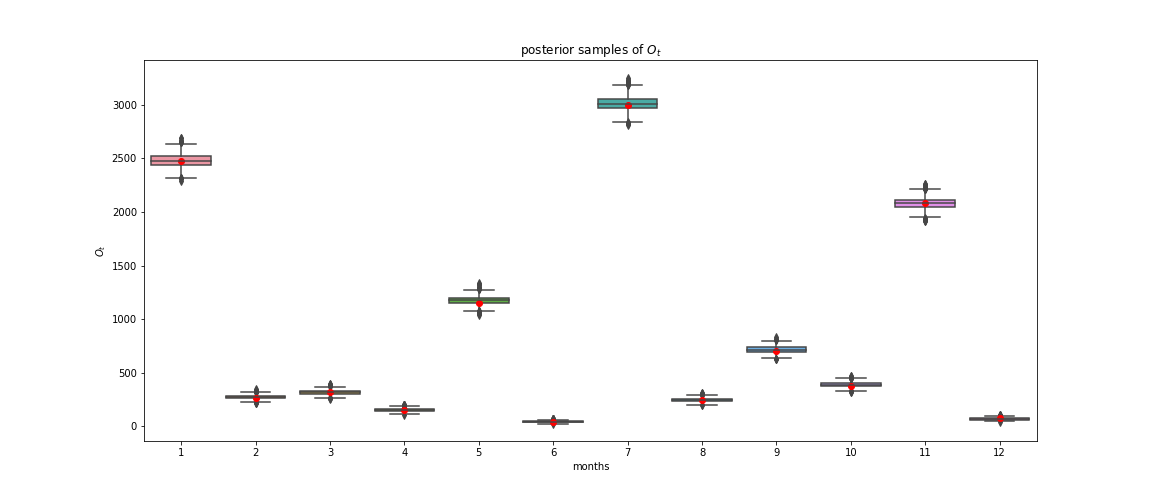
\includegraphics[width=1\linewidth]{Figures/earlyresult1_ot.png}
	\caption{Boxplot of posterior 2000 samples of $O_t$ with actual data as red dot.}
	\label{fig:screenshot001}
\end{figure}

 
\normalsize
%----------------------------------------------------------------------------------------
%	METHODS
%----------------------------------------------------------------------------------------

\section{template}
We first focus on the simplest sitaution that can describe the data sets and the general idea.

% \lipsum[5] % Dummy text

\begin{enumerate}[noitemsep] % [noitemsep] removes whitespace between the items for a compact look
\item First item in a list
\item Second item in a list
\item Third item in a list
\end{enumerate}

%------------------------------------------------

\subsection{Paragraphs}

%\lipsum[6] % Dummy text

\paragraph{Paragraph Description} %\lipsum[7] % Dummy text

\paragraph{Different Paragraph Description} %\lipsum[8] % Dummy text

%------------------------------------------------

\subsection{Math}

%\lipsum[4] % Dummy text

\begin{equation}
\cos^3 \theta =\frac{1}{4}\cos\theta+\frac{3}{4}\cos 3\theta
\label{eq:refname2}
\end{equation}

%\lipsum[5] % Dummy text

\begin{definition}[Gauss] 
To a mathematician it is obvious that
$\int_{-\infty}^{+\infty}
e^{-x^2}\,dx=\sqrt{\pi}$. 
\end{definition} 

\begin{theorem}[Pythagoras]
The square of the hypotenuse (the side opposite the right angle) is equal to the sum of the squares of the other two sides.
\end{theorem}

\begin{proof} 
We have that $\log(1)^2 = 2\log(1)$.
But we also have that $\log(-1)^2=\log(1)=0$.
Then $2\log(-1)=0$, from which the proof.
\end{proof}

%----------------------------------------------------------------------------------------
%	RESULTS AND DISCUSSION
%----------------------------------------------------------------------------------------

\section{Results and Discussion}

Reference to Figure~\vref{fig:gallery}. % The \vref command specifies the location of the reference

\begin{figure}[htb]
\centering 
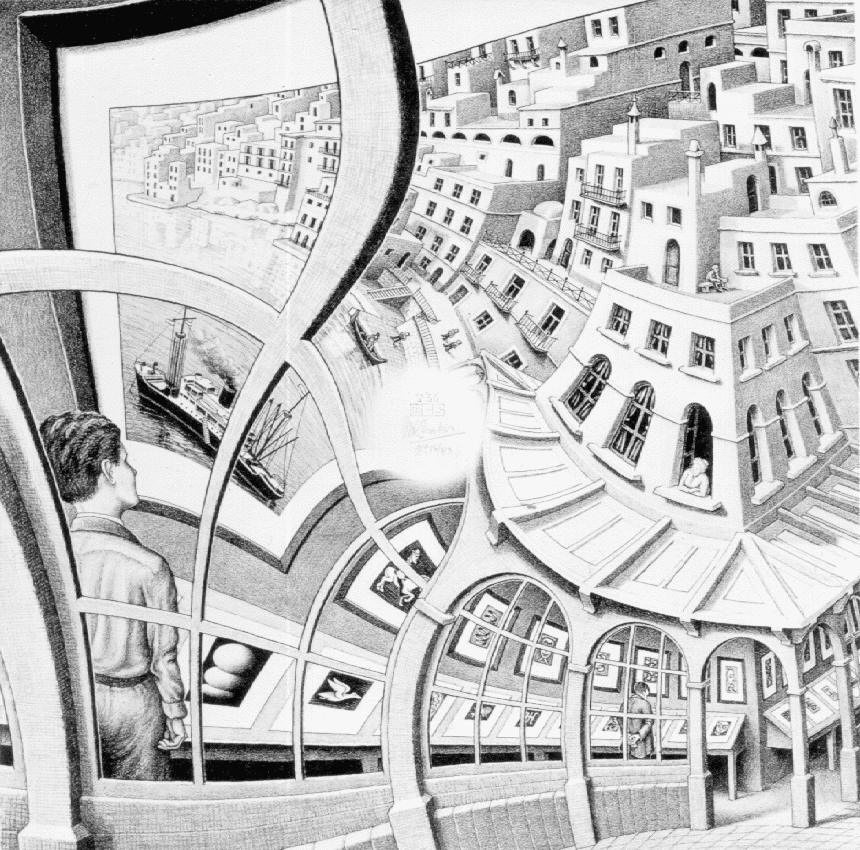
\includegraphics[width=0.5\columnwidth]{GalleriaStampe} 
\caption[An example of a floating figure]{An example of a floating figure (a reproduction from the \emph{Gallery of prints}, M.~Escher,\index{Escher, M.~C.} from \url{http://www.mcescher.com/}).} % The text in the square bracket is the caption for the list of figures while the text in the curly brackets is the figure caption
\label{fig:gallery} 
\end{figure}

%\lipsum[10] % Dummy text

%------------------------------------------------

\subsection{Subsection}

%\lipsum[11] % Dummy text

\subsubsection{Subsubsection}

%\lipsum[12] % Dummy text

\begin{description}
\item[Word] Definition
\item[Concept] Explanation
\item[Idea] Text
\end{description}

%\lipsum[12] % Dummy text

\begin{itemize}[noitemsep] % [noitemsep] removes whitespace between the items for a compact look
\item First item in a list
\item Second item in a list
\item Third item in a list
\end{itemize}

\subsubsection{Table}

%\lipsum[13] % Dummy text

\begin{table}[hbt]
\caption{Table of Grades}
\centering
\begin{tabular}{llr}
\toprule
\multicolumn{2}{c}{Name} \\
\cmidrule(r){1-2}
First name & Last Name & Grade \\
\midrule
John & Doe & $7.5$ \\
Richard & Miles & $2$ \\
\bottomrule
\end{tabular}
\label{tab:label}
\end{table}

Reference to Table~\vref{tab:label}. % The \vref command specifies the location of the reference

%------------------------------------------------

\subsection{Figure Composed of Subfigures}

Reference the figure composed of multiple subfigures as Figure~\vref{fig:esempio}. Reference one of the subfigures as Figure~\vref{fig:ipsum}. % The \vref command specifies the location of the reference

%\lipsum[15-18] % Dummy text

\begin{figure}[tb]
\centering
\subfloat[A city market.]{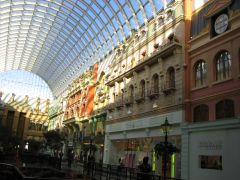
\includegraphics[width=.45\columnwidth]{Lorem}} \quad
\subfloat[Forest landscape.]{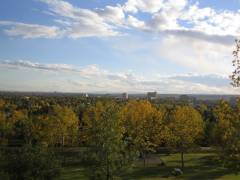
\includegraphics[width=.45\columnwidth]{Ipsum}\label{fig:ipsum}} \\
\subfloat[Mountain landscape.]{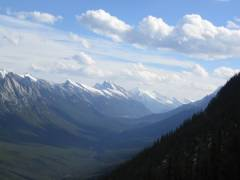
\includegraphics[width=.45\columnwidth]{Dolor}} \quad
\subfloat[A tile decoration.]{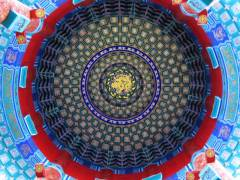
\includegraphics[width=.45\columnwidth]{Sit}}
\caption[A number of pictures.]{A number of pictures with no common theme.} % The text in the square bracket is the caption for the list of figures while the text in the curly brackets is the figure caption
\label{fig:esempio}
\end{figure}

%----------------------------------------------------------------------------------------
%	BIBLIOGRAPHY
%----------------------------------------------------------------------------------------

\renewcommand{\refname}{\spacedlowsmallcaps{References}} % For modifying the bibliography heading

\bibliographystyle{unsrt}

\bibliography{sample.bib} % The file containing the bibliography

%----------------------------------------------------------------------------------------

\end{document}